% Provenance (never printed): cycle 3 "Matiere, mouvement, energie,
% information" and "La planete Terre" (meteorological phenomena, the water in
% the air, measuring the weather); see sources/book1/PROVENANCE.md.
% Book 1, grade 4, chapter 1.
\chapter{Les nuages, la pluie et la neige}\label{ch:g4:clouds-rain-snow}

C'est un chaud après-midi d'été. À midi, le ciel était bleu, avec quelques
petits \omterm{def:g4:clouds-rain-snow:cloud}{nuages} blancs comme des boules de coton. Vers trois heures, l'un
d'eux a grandi. Il gonfle vers le haut, de plus en plus haut, comme un
chou-fleur blanc posé sur une base grise et plate. Son sommet s'étale. Sa
base devient sombre. Une rafale de vent frais souffle, les premières
grosses gouttes tombent, et pendant vingt minutes il pleut à verse. Puis le
\omterm{def:g4:clouds-rain-snow:cloud}{nuage} s'éloigne, le soleil revient, et les trottoirs mouillés fument.

D'où venait ce \omterm{def:g4:clouds-rain-snow:cloud}{nuage}~? De quoi est-il fait~? Et combien de \omterm{def:g4:clouds-rain-snow:precipitation}{pluie} est tombée
pendant ces vingt minutes~?

\begin{recall}
Le \omterm{def:g1:watching-the-weather:weather}{temps qu'il fait}, c'est l'état de l'air en un lieu et à un moment
donnés~: ensoleillé, nuageux, pluvieux, neigeux, venteux, brumeux~; nous le
notons dans un \omterm{def:g1:watching-the-weather:weather-chart}{tableau météo} (\cref{ch:g1:watching-the-weather}). L'eau de
la \omterm{def:g2:water-on-earth:ocean}{mer}, des \omterm{def:g1:landscapes-around-us:water}{lacs} et du sol monte dans l'air, puis retombe sous forme de
\omterm{def:g4:clouds-rain-snow:precipitation}{pluie} (\cref{ch:g2:water-on-earth}). Les livres de physique expliquent
comment l'eau s'évapore (de liquide, elle devient un gaz invisible), se
condense (de gaz, elle redevient de minuscules gouttes de liquide) et gèle
(de liquide, elle devient de la glace), et comment un thermomètre mesure la
température en degrés Celsius.
\end{recall}

\section{Qu'est-ce qu'un nuage~?}

L'air qui nous entoure contient toujours un peu d'eau, sous forme d'un gaz
invisible~: la vapeur d'eau. Quand l'air monte, il se refroidit. Quand il
s'est assez refroidi, une partie de sa vapeur d'eau se condense en
gouttelettes d'eau si minuscules que le moindre souffle d'air les maintient
en suspension. Des milliards de ces gouttelettes, \omterm{def:g1:landscapes-around-us:water}{côte} à \omterm{def:g1:landscapes-around-us:water}{côte}, forment un
\omterm{def:g4:clouds-rain-snow:cloud}{nuage} que nous pouvons voir. En altitude, là où l'air est très froid, les
gouttelettes gèlent, et le \omterm{def:g4:clouds-rain-snow:cloud}{nuage} est fait de minuscules morceaux de glace.

\begin{definition}[Nuage et brouillard]\label{def:g4:clouds-rain-snow:cloud}
Un \emph{nuage}\index{nuage} est un très grand nombre de minuscules
gouttelettes d'eau, ou de minuscules morceaux de glace, qui flottent
ensemble dans l'air. Le \emph{brouillard}\index{brouillard} est un nuage
qui touche le sol.
\end{definition}

\begin{example}[Ton haleine un matin froid]\label{ex:g4:clouds-rain-snow:breath}
Un matin froid, ton haleine fait un petit \omterm{def:g4:clouds-rain-snow:cloud}{nuage} blanc devant ta bouche.
L'air que tu expires est chaud et contient de la vapeur d'eau. L'air froid
le refroidit aussitôt, la vapeur se condense en minuscules gouttelettes ---
et un \omterm{def:g4:clouds-rain-snow:cloud}{nuage} miniature apparaît, puis disparaît quand les gouttelettes
s'évaporent de nouveau.
\end{example}

Un \omterm{def:g4:clouds-rain-snow:cloud}{nuage} est blanc parce que ses gouttelettes renvoient la lumière du
Soleil dans toutes les directions. Quand il est très épais, peu de lumière
parvient jusqu'à sa base, et vu d'en dessous il paraît gris, ou presque
noir~: c'est le signe d'un \omterm{def:g4:clouds-rain-snow:cloud}{nuage} lourd, chargé d'eau.

\section{Les familles de nuages}

Les \omterm{def:g4:clouds-rain-snow:cloud}{nuages} prennent bien des formes, et les observateurs du temps du monde
entier les classent de la même manière, d'après leur forme et la hauteur
à laquelle ils flottent.

\begin{definition}[Familles de nuages]\label{def:g4:clouds-rain-snow:cloud-families}
Les quatre familles de \omterm{def:g4:clouds-rain-snow:cloud}{nuages} à connaître sont~:
\begin{itemize}
  \item les \emph{cumulus}\index{cumulus}~: des \omterm{def:g4:clouds-rain-snow:cloud}{nuages} en tas, blancs et
        gonflés, à la base plate, comme des boules de coton~;
  \item les \emph{stratus}\index{stratus}~: des \omterm{def:g4:clouds-rain-snow:cloud}{nuages} en couche, une nappe
        grise et plate qui couvre tout le ciel, à basse altitude~;
  \item les \emph{cirrus}\index{cirrus}~: des \omterm{def:g4:clouds-rain-snow:cloud}{nuages} en filaments, de
        fins fils blancs ou des boucles, très hauts, faits de glace~;
  \item le \emph{cumulonimbus}\index{cumulonimbus}~: le \omterm{def:g4:clouds-rain-snow:cloud}{nuage} d'orage, une
        tour immense qui s'élève d'une base basse et sombre jusqu'à une très
        grande hauteur, et dont le sommet s'étale souvent à plat.
\end{itemize}
\end{definition}

Ces noms sont des mots latins~: \emph{\omterm{def:g4:clouds-rain-snow:cloud-families}{cumulus}} veut dire un tas,
\emph{\omterm{def:g4:clouds-rain-snow:cloud-families}{stratus}} une couche, \emph{\omterm{def:g4:clouds-rain-snow:cloud-families}{cirrus}} une boucle de cheveux, et
\emph{nimbus} un \omterm{def:g4:clouds-rain-snow:cloud}{nuage} de \omterm{def:g4:clouds-rain-snow:precipitation}{pluie}.

\begin{omfigure}
\begin{minipage}[b]{0.49\linewidth}\centering
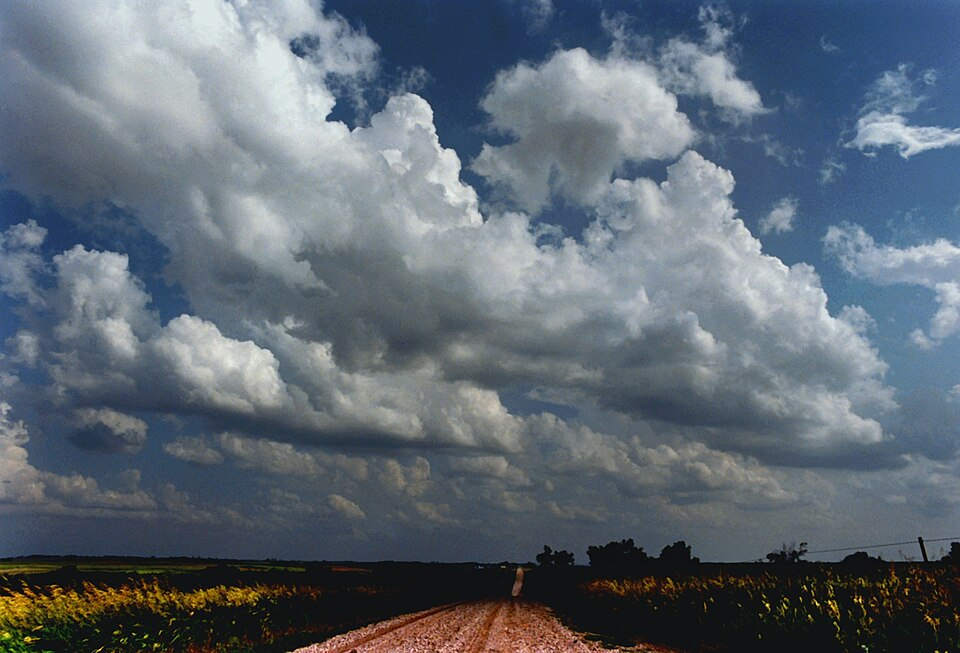
\includegraphics[width=\linewidth]{images/book1/g4-cumulus.jpg}

{\small Des \omterm{def:g4:clouds-rain-snow:cloud-families}{cumulus}, \omterm{def:g4:clouds-rain-snow:cloud}{nuages} en tas à la base plate.}
\end{minipage}\hfill
\begin{minipage}[b]{0.49\linewidth}\centering
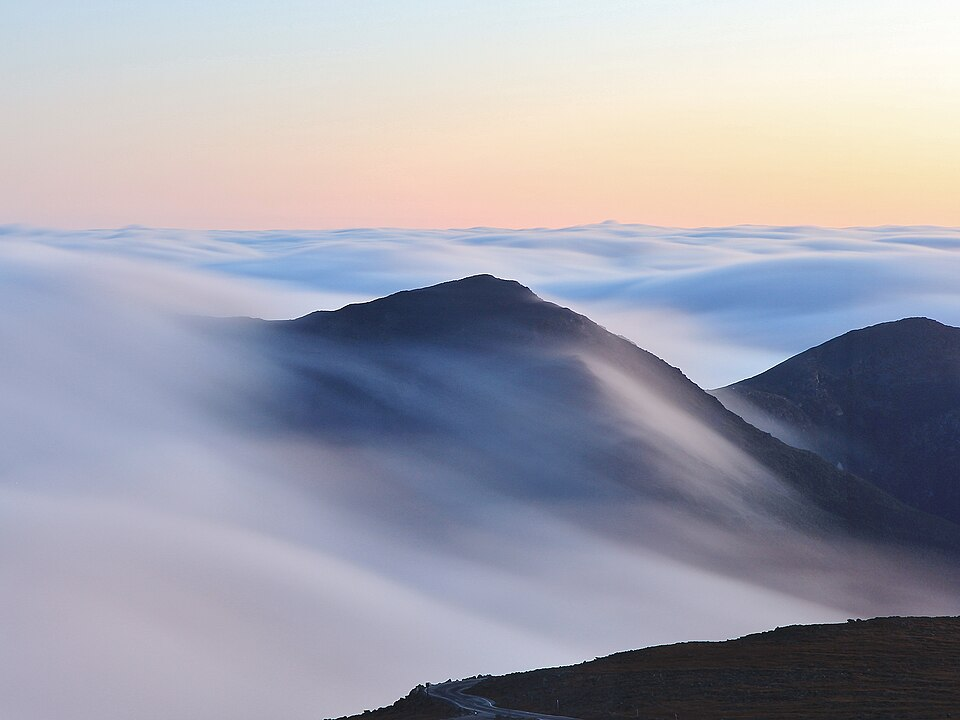
\includegraphics[width=\linewidth]{images/book1/g4-stratus.jpg}

{\small Des \omterm{def:g4:clouds-rain-snow:cloud-families}{stratus}~: une couche plate, vue ici d'en haut, depuis une \omterm{def:g1:landscapes-around-us:landform}{montagne}.}
\end{minipage}

\medskip
\begin{minipage}[b]{0.49\linewidth}\centering
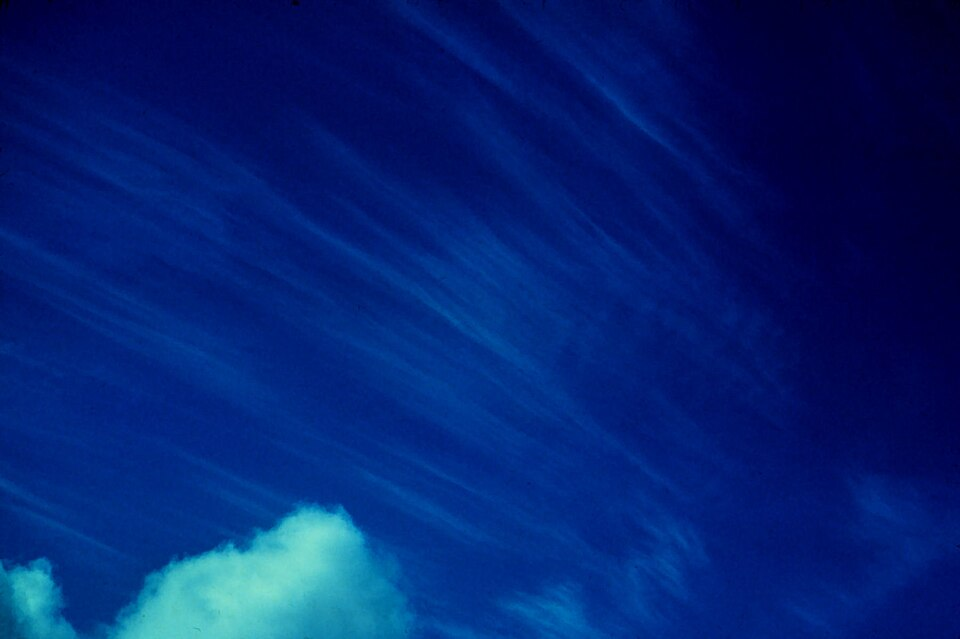
\includegraphics[width=\linewidth]{images/book1/g4-cirrus.jpg}

{\small Des \omterm{def:g4:clouds-rain-snow:cloud-families}{cirrus}~: de fins fils de glace, très hauts (un petit \omterm{def:g4:clouds-rain-snow:cloud-families}{cumulus} en dessous).}
\end{minipage}\hfill
\begin{minipage}[b]{0.49\linewidth}\centering
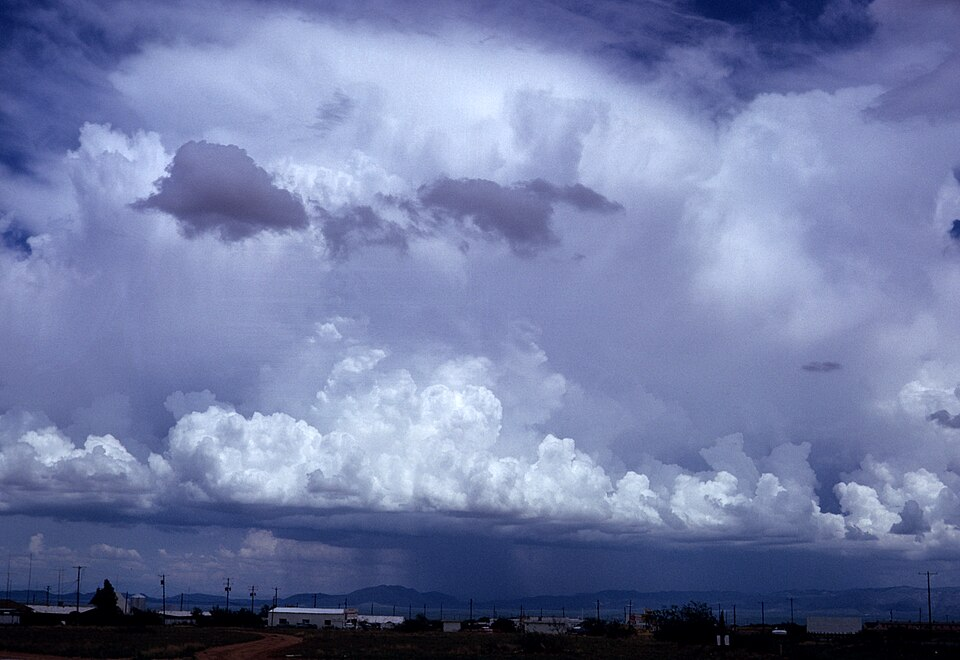
\includegraphics[width=\linewidth]{images/book1/g4-cumulonimbus.jpg}

{\small Un \omterm{def:g4:clouds-rain-snow:cloud-families}{cumulonimbus}~: une tour de \omterm{def:g4:clouds-rain-snow:cloud}{nuage}~; la \omterm{def:g4:clouds-rain-snow:precipitation}{pluie} tombe de sa base sombre.}
\end{minipage}

\smallskip
{\small Photographies~: NOAA Photo Library (domaine public)~: S. Corfidi
(\omterm{def:g4:clouds-rain-snow:cloud-families}{cumulus}), R. F. Kresge (\omterm{def:g4:clouds-rain-snow:cloud-families}{cirrus}), collection B. Hooke (\omterm{def:g4:clouds-rain-snow:cloud-families}{cumulonimbus}).}
% ledger: noaa:photos-g4
\label{fig:g4:clouds-rain-snow:photos}
\end{omfigure}

À quelle hauteur flottent les \omterm{def:g4:clouds-rain-snow:cloud}{nuages}~? Cela dépend de leur famille. Les
\omterm{def:g4:clouds-rain-snow:cloud}{nuages} bas, comme les \omterm{def:g4:clouds-rain-snow:cloud-families}{stratus} et la base des \omterm{def:g4:clouds-rain-snow:cloud-families}{cumulus}, flottent depuis à
peine au-dessus du sol jusqu'à environ 2 kilomètres. Les \omterm{def:g4:clouds-rain-snow:cloud-families}{cirrus} flottent
très haut, entre environ 5 et 13 kilomètres en dehors des tropiques et des
régions polaires --- souvent plus haut que la plus haute \omterm{def:g1:landscapes-around-us:landform}{montagne} de la
Terre. Un \omterm{def:g4:clouds-rain-snow:cloud-families}{cumulonimbus} s'étend depuis une base basse jusqu'au sommet même
des étages de \omterm{def:g4:clouds-rain-snow:cloud}{nuages}.
% ledger: wmo:cloud-levels, wmo:cumulonimbus

\begin{omfigure}
\begin{tikzpicture}[x=1cm, y=0.5cm, font=\small]
  % height scale
  \draw[black!60] (0,0) -- (0,14);
  \foreach \h in {0,2,...,14} {
    \draw[black!60] (-0.1,\h) -- (0,\h);
    \node[anchor=east, font=\scriptsize] at (-0.12,\h) {\h\,km};
  }
  \node[anchor=south, font=\scriptsize, align=center] at (0,14.2) {altitude};
  % ground and a mountain for comparison
  \fill[green!35!black!50] (0.2,0) -- (11.4,0) -- (11.4,-0.4) -- (0.2,-0.4) -- cycle;
  \fill[black!35] (8.6,0) -- (9.9,8.8) -- (10.2,8.4) -- (11.2,0) -- cycle;
  \fill[white, draw=black!45, line width=0.3pt] (9.65,7.2) -- (9.9,8.8) -- (10.2,8.4) -- (10.4,7.0) -- (10.1,7.4) -- (9.9,7.0) -- cycle;
  \node[font=\scriptsize, align=center] at (9.9,10.2) {la plus haute\\montagne};
  % levels
  \fill[blue!6] (0.2,0.15) rectangle (8.3,2);
  \fill[blue!10] (0.2,5) rectangle (8.3,13);
  \node[anchor=west, font=\scriptsize, text=blue!50!black] at (0.3,1.65) {nuages bas};
  \node[anchor=west, font=\scriptsize, text=blue!50!black] at (0.3,12.6) {nuages hauts};
  % stratus: a flat grey layer
  \fill[black!25, rounded corners=2pt] (0.6,0.6) rectangle (2.6,1.3);
  \node[font=\scriptsize] at (1.6,-1.1) {stratus};
  % cumulus
  \pic[scale=0.7, transform shape] at (4.0,0.9) {puffycloud};
  \node[font=\scriptsize] at (4.0,-1.1) {cumulus};
  % cirrus: wisps
  \foreach \y in {9.4,10.0,10.6} {
    \draw[black!50, line width=0.6pt] (0.8,\y) .. controls (1.4,\y+0.5) and (2.0,\y+0.1) .. (2.6,\y+0.6);
  }
  \node[font=\scriptsize] at (1.7,8.5) {cirrus};
  % cumulonimbus: tower with an anvil
  \fill[black!15, draw=black!45, line width=0.4pt]
    (5.4,1.0) .. controls (5.2,4) and (5.6,8) .. (5.9,11.2)
    .. controls (5.0,11.6) and (4.6,12.0) .. (4.8,12.3)
    -- (8.1,12.3) .. controls (8.2,12.0) and (7.8,11.6) .. (7.0,11.2)
    .. controls (7.3,8) and (7.6,4) .. (7.4,1.0) -- cycle;
  \fill[black!45] (5.4,1.0) rectangle (7.4,1.4);
  \foreach \x in {5.7,6.1,6.5,6.9,7.2}
    \draw[omWxRain, line width=0.6pt] (\x,0.95) -- (\x-0.15,0.15);
  \node[font=\scriptsize] at (6.4,-1.1) {cumulonimbus};
\end{tikzpicture}

{\small À quelle hauteur flottent les quatre familles de \omterm{def:g4:clouds-rain-snow:cloud}{nuages} (hauteurs
en kilomètres, pour les régions qui ne sont ni tropicales ni polaires). Les
\omterm{def:g4:clouds-rain-snow:cloud-families}{stratus} et la base des \omterm{def:g4:clouds-rain-snow:cloud-families}{cumulus} sont bas~; les \omterm{def:g4:clouds-rain-snow:cloud-families}{cirrus} sont souvent plus
hauts que la plus haute \omterm{def:g1:landscapes-around-us:landform}{montagne}. Un \omterm{def:g4:clouds-rain-snow:cloud-families}{cumulonimbus} s'étend d'une base basse
jusqu'au sommet des étages de \omterm{def:g4:clouds-rain-snow:cloud}{nuages}. Hauteurs d'après l'atlas des \omterm{def:g4:clouds-rain-snow:cloud}{nuages}
de l'Organisation météorologique mondiale.}
\label{fig:g4:clouds-rain-snow:heights}
% ledger: wmo:cloud-levels, tht:everest
\end{omfigure}

\begin{method}[Nommer un nuage]\label{met:g4:clouds-rain-snow:naming}
Regarde le ciel et pose-toi trois questions~:
\begin{enumerate}
  \item Est-ce un tas à la base plate~? Alors c'est un \omterm{def:g4:clouds-rain-snow:cloud-families}{cumulus} --- et s'il
        s'élève en une immense tour sombre, un \omterm{def:g4:clouds-rain-snow:cloud-families}{cumulonimbus}.
  \item Est-ce une nappe plate et régulière qui cache tout le ciel~? Alors
        c'est un \omterm{def:g4:clouds-rain-snow:cloud-families}{stratus}.
  \item Est-il fait de fins fils blancs, très hauts~? Alors c'est un \omterm{def:g4:clouds-rain-snow:cloud-families}{cirrus}.
\end{enumerate}
\end{method}

\begin{remark}[Les nuages annoncent le temps]\label{rem:g4:clouds-rain-snow:tell}
De petits \omterm{def:g4:clouds-rain-snow:cloud-families}{cumulus} dans un ciel bleu annoncent le beau temps. Un \omterm{def:g4:clouds-rain-snow:cloud-families}{stratus}
gris apporte une journée terne, parfois avec de la bruine. Un \omterm{def:g4:clouds-rain-snow:cloud-families}{cumulonimbus}
apporte une averse courte et forte, souvent avec du tonnerre, des éclairs
et des rafales de vent --- parfois de la \omterm{def:g4:clouds-rain-snow:precipitation}{grêle}. Les \omterm{def:g4:clouds-rain-snow:cloud-families}{cirrus} n'apportent pas
de \omterm{def:g4:clouds-rain-snow:precipitation}{pluie}, mais quand ils s'étendent et s'épaississent, la \omterm{def:g4:clouds-rain-snow:precipitation}{pluie} suit
souvent un jour plus tard.
\end{remark}

\section{La pluie, la neige et la grêle}

À l'intérieur d'un \omterm{def:g4:clouds-rain-snow:cloud}{nuage}, les minuscules gouttelettes se heurtent et se
réunissent, ou bien des cristaux de glace grossissent aux dépens des
gouttelettes. Une goutte de \omterm{def:g4:clouds-rain-snow:cloud}{nuage}, ou un cristal, devenue assez grosse et
assez lourde ne peut plus flotter~: elle tombe.

\begin{definition}[Précipitations]\label{def:g4:clouds-rain-snow:precipitation}
Les \emph{précipitations}\index{precipitations@précipitations} sont l'eau
qui tombe d'un \omterm{def:g4:clouds-rain-snow:cloud}{nuage} jusqu'au sol~: la \emph{pluie}\index{pluie} (des
gouttes d'eau liquide), la \emph{neige}\index{neige} (des flocons faits de
cristaux de glace collés ensemble) ou la \emph{grêle}\index{grele@grêle}
(des billes de glace, appelées grêlons, qui tombent des \omterm{def:g4:clouds-rain-snow:cloud}{nuages} d'orage).
\end{definition}

Qu'il pleuve ou qu'il \omterm{def:g4:clouds-rain-snow:precipitation}{neige} dépend de la température de l'air que
traversent les \omterm{def:g4:clouds-rain-snow:precipitation}{précipitations}. Les flocons de \omterm{def:g4:clouds-rain-snow:precipitation}{neige} se forment en haut, dans
le \omterm{def:g4:clouds-rain-snow:cloud}{nuage} froid. Si l'air en dessous est au-dessus de \SI{0}{\celsius}
assez longtemps, ils fondent pendant leur chute et nous arrivent sous forme
de \omterm{def:g4:clouds-rain-snow:precipitation}{pluie}. Si l'air est sous zéro jusqu'au sol, ils arrivent sous forme de
\omterm{def:g4:clouds-rain-snow:precipitation}{neige}.

\begin{omfigure}

\includegraphics[width=0.55\linewidth]{images/book1/ai/g4-snowflakes.jpg}

{\small Des enfants attrapent des flocons de \omterm{def:g4:clouds-rain-snow:precipitation}{neige} sur un gant sombre~:
chaque flocon est fait de cristaux de glace.}
\end{omfigure}

La \omterm{def:g4:clouds-rain-snow:precipitation}{grêle} ne tombe que des \omterm{def:g4:clouds-rain-snow:cloud-families}{cumulonimbus}. À l'intérieur de la tour, de
puissants vents ascendants font monter et descendre des grains de glace
plusieurs fois~; chaque voyage ajoute une nouvelle couche de glace, comme
les couches d'un oignon, jusqu'à ce que le grêlon soit trop lourd pour que
le vent le retienne.

\begin{omfigure}
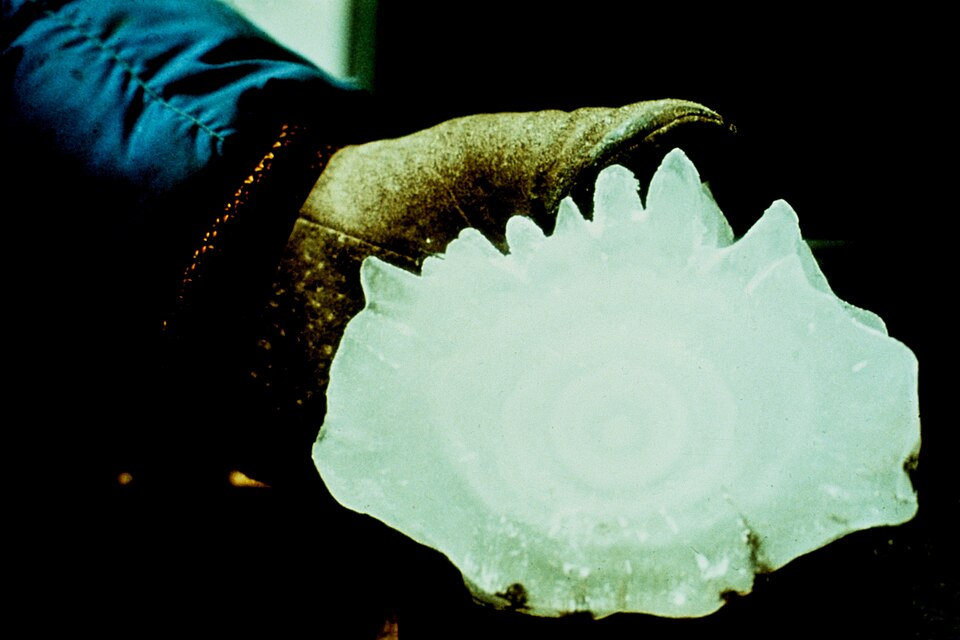
\includegraphics[width=0.5\linewidth]{images/book1/g4-hailstone.jpg}

{\small Un très gros grêlon tenu dans une main gantée. Les anneaux montrent
les couches de glace qu'il a accumulées dans le \omterm{def:g4:clouds-rain-snow:cloud}{nuage} d'orage.
Photographie~: NOAA Photo Library (domaine public).}
% ledger: noaa:photos-g4
\end{omfigure}

\section{Mesurer le temps qu'il fait}

Pour dire combien il a plu, quelle température il faisait ou d'où soufflait
le vent, les mots ne suffisent pas~: il nous faut des instruments, et des
nombres.

\begin{definition}[Pluviomètre]\label{def:g4:clouds-rain-snow:rain-gauge}
Un \emph{pluviomètre}\index{pluviometre@pluviomètre} est un récipient qui
recueille la \omterm{def:g4:clouds-rain-snow:precipitation}{pluie} tombant sur son ouverture. La hauteur d'eau recueillie
se mesure en millimètres~: «~5 millimètres de \omterm{def:g4:clouds-rain-snow:precipitation}{pluie}~» veut dire que la \omterm{def:g4:clouds-rain-snow:precipitation}{pluie}
aurait formé une couche d'eau de 5 millimètres d'épaisseur sur un sol
plat, si rien n'avait ruisselé ni ne s'était infiltré.
\end{definition}

\begin{remark}[Un millimètre de pluie, c'est beaucoup d'eau]\label{rem:g4:clouds-rain-snow:litre}
Un millimètre de \omterm{def:g4:clouds-rain-snow:precipitation}{pluie} paraît minuscule dans le \omterm{def:g4:clouds-rain-snow:rain-gauge}{pluviomètre}. Mais sur un
carré de sol d'un mètre sur un mètre, cela fait un litre d'eau~: une
grande bouteille. Sur une cour d'école de mille mètres carrés, une \omterm{def:g4:clouds-rain-snow:precipitation}{pluie} de
10 millimètres apporte dix mille litres~: de quoi remplir mille seaux de
10 litres chacun.
\end{remark}

\begin{omfigure}
\begin{tikzpicture}[font=\small]
  % funnel
  \draw[black!70, line width=0.8pt] (-1.2,6.6) -- (-0.35,5.8) -- (-0.35,5.4);
  \draw[black!70, line width=0.8pt] (1.2,6.6) -- (0.35,5.8) -- (0.35,5.4);
  \draw[black!70, line width=0.8pt] (-1.2,6.6) -- (1.2,6.6);
  % tube
  \fill[blue!25] (-0.45,0) rectangle (0.45,2.4);
  \draw[black!70, line width=0.8pt] (-0.45,5.4) -- (-0.45,0) -- (0.45,0) -- (0.45,5.4);
  \foreach \m in {0,1,...,50} {
    \pgfmathsetmacro{\yy}{\m*0.1}
    \draw[black!60] (0.45,\yy) -- ++(-0.12,0);
  }
  \foreach \m in {0,5,10,...,50} {
    \pgfmathsetmacro{\yy}{\m*0.1}
    \draw[black!80] (0.45,\yy) -- ++(-0.25,0);
    \node[anchor=west, font=\scriptsize] at (0.5,\yy) {\m};
  }
  \node[anchor=west, font=\scriptsize] at (1.0,5.0) {mm};
  % reading line
  \draw[red!70!black, -{Stealth}] (-1.6,2.4) -- (-0.5,2.4);
  \node[anchor=east, align=right, font=\scriptsize] at (-1.65,2.4) {lis le\\niveau ici};
  \node[anchor=west, font=\scriptsize] at (1.9,2.4) {$\leftarrow$ 24\,mm de pluie};
\end{tikzpicture}

{\small Un \omterm{def:g4:clouds-rain-snow:rain-gauge}{pluviomètre} simple~: un entonnoir recueille la \omterm{def:g4:clouds-rain-snow:precipitation}{pluie} et un tube
gradué en millimètres la garde. Lis le niveau de l'eau, l'œil à la même
hauteur. Ici, 24 millimètres sont tombés depuis que le \omterm{def:g4:clouds-rain-snow:rain-gauge}{pluviomètre} a été
vidé pour la dernière fois.}
\label{fig:g4:clouds-rain-snow:gauge}
\end{omfigure}


\begin{definition}[Girouette]\label{def:g4:clouds-rain-snow:wind-vane}
Une \emph{girouette}\index{girouette} est une flèche qui tourne librement
sur un mât. Le vent pousse sa queue, si bien que la flèche montre toujours
la direction \emph{d'où} vient le vent.
\end{definition}

\begin{definition}[Station météo]\label{def:g4:clouds-rain-snow:weather-station}
Une \emph{station météo}\index{station meteo@station météo} est un lieu où
l'on mesure le \omterm{def:g1:watching-the-weather:weather}{temps qu'il fait} chaque jour, toujours de la même façon,
avec des instruments~: un thermomètre dans un abri blanc aéré, un
\omterm{def:g4:clouds-rain-snow:rain-gauge}{pluviomètre} à découvert, une \omterm{def:g4:clouds-rain-snow:wind-vane}{girouette} sur un mât.
\end{definition}

Le thermomètre est gardé à l'ombre, dans un abri blanc aux parois à
lamelles qui laissent passer l'air mais arrêtent le soleil et la \omterm{def:g4:clouds-rain-snow:precipitation}{pluie}. Le
Met Office, le service \omterm{def:g1:watching-the-weather:weather}{météorologique} du Royaume-Uni, le place à
\SI{1.25}{\metre} au-dessus du sol. Le \omterm{def:g4:clouds-rain-snow:rain-gauge}{pluviomètre}
est installé à découvert, loin des murs et des arbres qui l'abriteraient de
la \omterm{def:g4:clouds-rain-snow:precipitation}{pluie}, son ouverture un peu au-dessus du sol. La \omterm{def:g4:clouds-rain-snow:wind-vane}{girouette} est en haut
de son mât, au-dessus des obstacles qui dévieraient le vent.
% ledger: mo:screen-height, mo:raingauge

\begin{omfigure}
\begin{tikzpicture}[font=\small, x=1cm, y=1cm]
  % grass
  \fill[green!40!black!45] (-0.5,0) rectangle (11,-0.25);
  \foreach \x in {-0.3,0.1,...,10.8} \draw[green!45!black] (\x,0) -- ++(0.06,0.14);
  % screen on legs
  \draw[black!70, line width=1pt] (0.8,0) -- (0.8,1.25) (2.2,0) -- (2.2,1.25);
  \fill[white, draw=black!70] (0.6,1.25) rectangle (2.4,2.4);
  \foreach \y in {1.4,1.55,...,2.25} \draw[black!40] (0.7,\y) -- (2.3,\y-0.08);
  \fill[white, draw=black!70] (0.45,2.4) -- (1.5,2.75) -- (2.55,2.4) -- cycle;
  \draw[black!60, <->] (2.8,0) -- node[right, font=\scriptsize, align=left] {environ\\1.25\,m} (2.8,1.25);
  \node[align=center, font=\scriptsize] at (1.5,3.25) {thermomètre dans un\\abri blanc à lamelles};
  % rain gauge
  \fill[black!15, draw=black!70] (5.4,0) rectangle (5.9,0.4);
  \draw[black!70] (5.3,0.55) -- (5.4,0.4) (6.0,0.55) -- (5.9,0.4);
  \node[align=center, font=\scriptsize] at (5.65,1.2) {pluviomètre,\\à découvert};
  % tree far away
  \fill[brown!60!black] (7.3,0) rectangle (7.5,1.3);
  \fill[green!50!black!70] (7.4,2.1) circle (0.85);
  % wind vane on a mast
  \draw[black!70, line width=1pt] (9.8,0) -- (9.8,4.2);
  \draw[black!80, line width=1.4pt, -{Latex[length=3mm]}] (10.6,4.4) -- (9.0,4.4);
  \fill[black!80] (10.6,4.4) -- (10.9,4.65) -- (10.9,4.15) -- cycle;
  \node[align=center, font=\scriptsize] at (9.8,5.05) {girouette sur un haut mât};
  \node[anchor=west, font=\scriptsize, align=left] at (10.1,3.4) {montre d'où\\vient le vent};
\end{tikzpicture}

{\small Une petite \omterm{def:g4:clouds-rain-snow:weather-station}{station météo}. Le thermomètre est à l'ombre, dans un
abri blanc aux parois à lamelles, à environ 1.25 mètre au-dessus de
l'herbe~; le \omterm{def:g4:clouds-rain-snow:rain-gauge}{pluviomètre} est à découvert, loin de l'arbre~; la \omterm{def:g4:clouds-rain-snow:wind-vane}{girouette}
est haut au-dessus des obstacles.}
\label{fig:g4:clouds-rain-snow:station}
% ledger: mo:screen-height
\end{omfigure}

\begin{inthefield}[Une station météo dans la cour de l'école]
Beaucoup d'écoles ont une petite \omterm{def:g4:clouds-rain-snow:weather-station}{station météo} dans un coin de la cour.
Chaque matin à la même heure, deux élèves lisent le thermomètre, lisent et
vident le \omterm{def:g4:clouds-rain-snow:rain-gauge}{pluviomètre}, et notent où pointe la \omterm{def:g4:clouds-rain-snow:wind-vane}{girouette}. Semaine après
semaine, la classe constitue un relevé de son propre temps.
\end{inthefield}

\begin{omfigure}
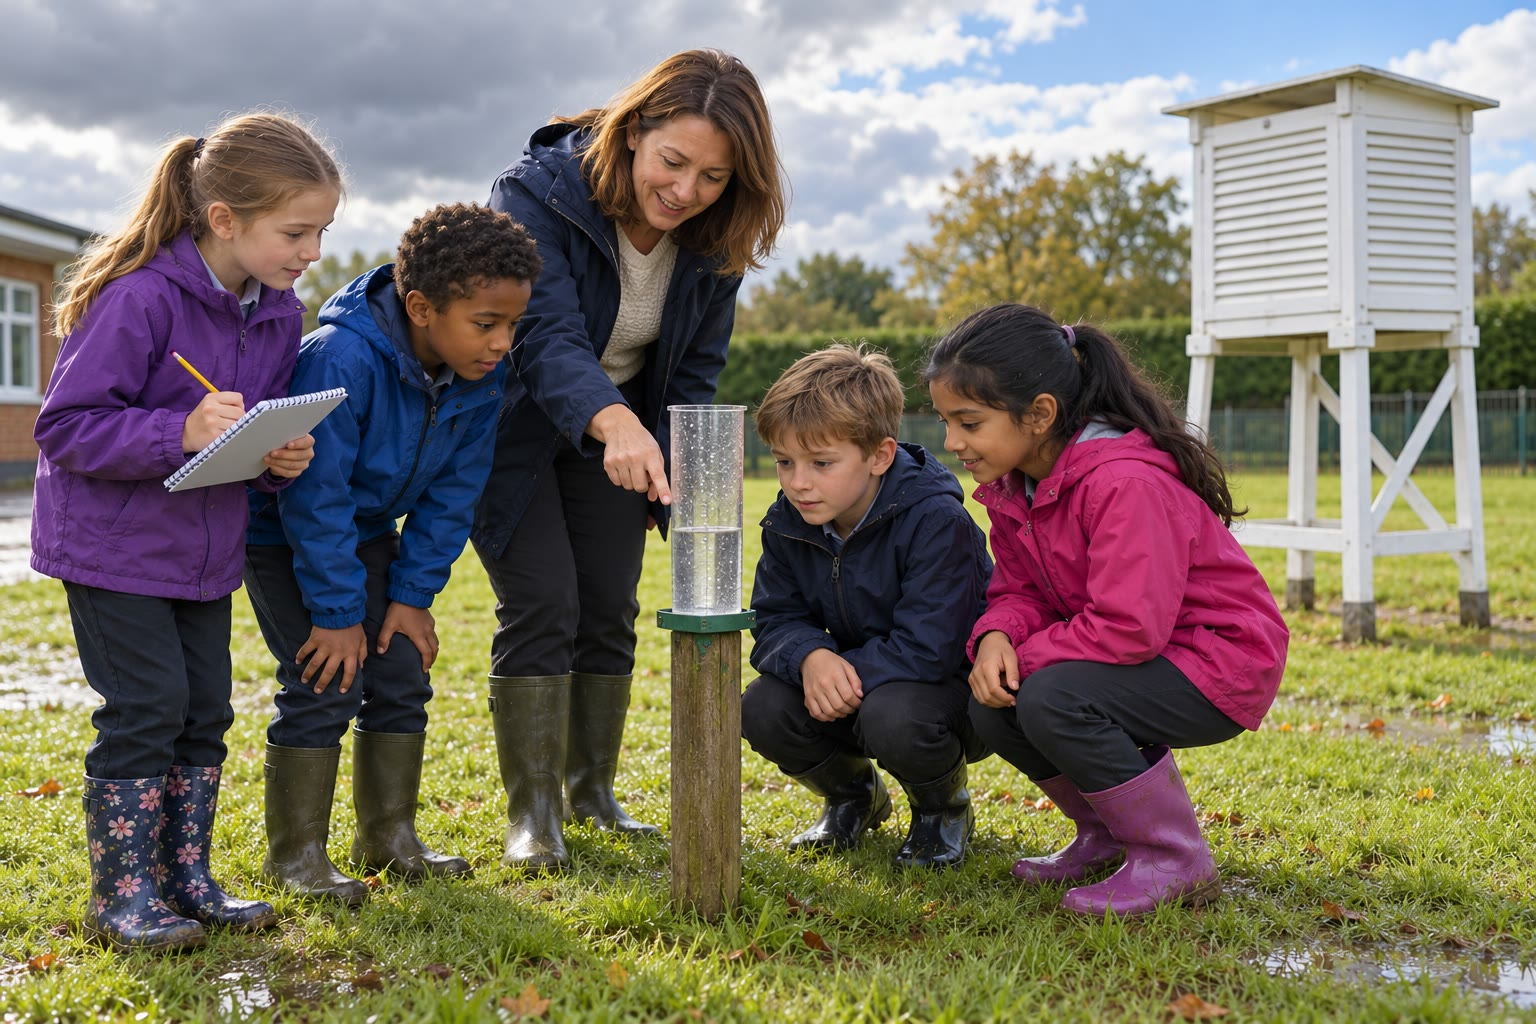
\includegraphics[width=0.55\linewidth]{images/book1/ai/g4-rain-gauge-class.jpg}

{\small Des élèves lisent le \omterm{def:g4:clouds-rain-snow:rain-gauge}{pluviomètre} dans la cour de l'école.}
\end{omfigure}

\begin{method}[Tracer un diagramme en bâtons de la pluie]\label{met:g4:clouds-rain-snow:bar-chart}
Pour représenter la \omterm{def:g4:clouds-rain-snow:precipitation}{pluie} d'une semaine~:
\begin{enumerate}
  \item trace une ligne horizontale et écris les jours dessous, à
        intervalles réguliers~;
  \item trace une ligne verticale à gauche et gradue-la en millimètres, avec
        des pas égaux (par exemple tous les 2 millimètres)~;
  \item au-dessus de chaque jour, dessine un bâton aussi haut que la \omterm{def:g4:clouds-rain-snow:precipitation}{pluie}
        de ce jour~; un jour sans \omterm{def:g4:clouds-rain-snow:precipitation}{pluie} n'a pas de bâton du tout~;
  \item donne un titre au diagramme et écris l'unité, mm, sur la ligne
        verticale.
\end{enumerate}
\end{method}

\begin{example}[Une semaine de pluie à l'école]\label{ex:g4:clouds-rain-snow:week}
La classe a lu le \omterm{def:g4:clouds-rain-snow:rain-gauge}{pluviomètre} chaque matin pendant une semaine et a
trouvé~: lundi 0, mardi 4, mercredi 12, jeudi 7, vendredi 0, samedi 2,
dimanche 5 millimètres. Le jour le plus pluvieux a été mercredi. Il n'a
plu ni lundi ni vendredi. Sur toute la semaine,
$0 + 4 + 12 + 7 + 0 + 2 + 5 = 30$ millimètres sont tombés. Mercredi, à lui
seul, a apporté 12 des 30 millimètres, soit
$\frac{12}{30} = \frac{2}{5}$ de la \omterm{def:g4:clouds-rain-snow:precipitation}{pluie} de la semaine.
\end{example}

\begin{omfigure}
\begin{tikzpicture}
\begin{axis}[ybar, bar width=14pt, width=0.8\linewidth, height=5.4cm,
    ymin=0, ymax=14, ytick={0,2,...,14}, ylabel={pluie (mm)},
    symbolic x coords={Mon,Tue,Wed,Thu,Fri,Sat,Sun}, xtick=data, xticklabels={lun.,mar.,mer.,jeu.,ven.,sam.,dim.},
    axis x line*=bottom, axis y line*=left, ymajorgrids, grid style={gray!25},
    nodes near coords, nodes near coords style={font=\scriptsize},
    every axis label/.append style={font=\small}, tick label style={font=\small},
    title={La pluie à l'école pendant une semaine}, title style={font=\small}]
  \addplot[fill=omWxRain!70, draw=omWxRain!60!black] coordinates
    {(Mon,0) (Tue,4) (Wed,12) (Thu,7) (Fri,0) (Sat,2) (Sun,5)};
\end{axis}
\end{tikzpicture}

{\small La semaine de l'\cref{ex:g4:clouds-rain-snow:week} en diagramme en bâtons.}
\label{fig:g4:clouds-rain-snow:bars}
\end{omfigure}

\section{Exercices}

\begin{exercise}[$\star$]\label{exo:g4:clouds-rain-snow:1}
De quoi est fait un \omterm{def:g4:clouds-rain-snow:cloud}{nuage}~? Qu'est-ce que le \omterm{def:g4:clouds-rain-snow:cloud}{brouillard}~?
\end{exercise}

\begin{exercise}[$\star$]\label{exo:g4:clouds-rain-snow:2}
Nomme le \omterm{def:g4:clouds-rain-snow:cloud}{nuage}~: (a) une nappe grise et plate qui cache tout le ciel~;
(b) de fins fils blancs très hauts dans un ciel bleu~; (c) des tas blancs à
la base plate, comme du coton~; (d) une immense tour sombre au sommet
plat, qui apporte le tonnerre.
\end{exercise}

\begin{exercise}[$\star$]\label{exo:g4:clouds-rain-snow:3}
\omterm{def:g4:clouds-rain-snow:precipitation}{Pluie}, \omterm{def:g4:clouds-rain-snow:precipitation}{neige} ou \omterm{def:g4:clouds-rain-snow:precipitation}{grêle}~? (a) des billes de glace qui tombent d'un \omterm{def:g4:clouds-rain-snow:cloud}{nuage}
d'orage~; (b) des gouttes d'eau liquide~; (c) des flocons faits de cristaux
de glace.
\end{exercise}

\begin{exercise}[$\star$]\label{exo:g4:clouds-rain-snow:4}
Quel instrument mesure~: (a) la \omterm{def:g4:clouds-rain-snow:precipitation}{pluie}~; (b) la température~; (c) d'où vient
le vent~?
\end{exercise}

\begin{exercise}[$\star$]\label{exo:g4:clouds-rain-snow:5}
Dans le \omterm{def:g4:clouds-rain-snow:rain-gauge}{pluviomètre} dessiné page~\pageref{fig:g4:clouds-rain-snow:gauge},
l'eau atteint maintenant la graduation 17. Combien de millimètres de \omterm{def:g4:clouds-rain-snow:precipitation}{pluie}
sont tombés~? Combien de millimètres de plus l'amèneraient à 20~?
\end{exercise}

\begin{exercise}[$\star$]\label{exo:g4:clouds-rain-snow:6}
Regarde le diagramme en bâtons de la page~\pageref{fig:g4:clouds-rain-snow:bars}.
Quel jour a été le plus pluvieux~? Quels jours n'a-t-il pas plu~? Quel
jour a eu 7 millimètres~?
\end{exercise}

\begin{exercise}[$\star\star$]\label{exo:g4:clouds-rain-snow:7}
Un matin de \omterm{def:g4:clouds-rain-snow:precipitation}{neige}, les flocons arrivent jusqu'au sol dans le village de
\omterm{def:g1:landscapes-around-us:landform}{montagne}, mais dans la \omterm{def:g1:landscapes-around-us:landform}{vallée} en contrebas il pleut. Explique la
différence à l'aide de la température de l'air.
\end{exercise}

\begin{exercise}[$\star\star$]\label{exo:g4:clouds-rain-snow:8}
Une autre semaine, la classe trouve~: lundi 3, mardi 0, mercredi 1,
jeudi 9, vendredi 6, samedi 0, dimanche 1 millimètre. Trace le diagramme
en bâtons. Combien de millimètres sont tombés dans la semaine~? Quelle
fraction de la \omterm{def:g4:clouds-rain-snow:precipitation}{pluie} de la semaine est tombée jeudi~?
\end{exercise}

\begin{exercise}[$\star\star$]\label{exo:g4:clouds-rain-snow:9}
Pourquoi le \omterm{def:g4:clouds-rain-snow:rain-gauge}{pluviomètre} doit-il être à découvert, loin des murs et des
arbres~? Pourquoi garde-t-on le thermomètre dans un abri blanc à l'ombre,
et non en plein soleil~?
\end{exercise}

\begin{exercise}[$\star\star$]\label{exo:g4:clouds-rain-snow:10}
La \omterm{def:g4:clouds-rain-snow:wind-vane}{girouette} montre l'ouest. D'où vient le vent~? Où va-t-il~?
\end{exercise}

\begin{exercise}[$\star\star\star$]\label{exo:g4:clouds-rain-snow:11}
Sur une cour de 500 mètres carrés, il tombe 8 millimètres de \omterm{def:g4:clouds-rain-snow:precipitation}{pluie}. À
l'aide de la \cref{rem:g4:clouds-rain-snow:litre}, combien de litres d'eau
sont tombés sur la cour~? Un arrosoir contient 10 litres~: combien
d'arrosoirs cela fait-il~?
\end{exercise}
